%---------------------------------------------------------
% Chapter: A chapter about figures and tables
%----------------------------------------------------------
\chapter{Figures and Tables}
\label{chap:FIGURESANDTABLES}

\section{Floats}

A \emph{float} is an object in a document that should not be broken across
multiple pages. The term ``float'' signifies that \LaTeX\ may move
a floating object within the document to preserve the flow of the
document (e.g., to ensure that the bottom of a page doesn't have a
gaping hole simply because the figure does not fit on the page) and to
improve the alignment of the object if more than one can fit
horizontally on the page.

Understanding what \LaTeX\ will do with a float is important
because the system will make decisions about where to place
a float automatically; the position of the float in your
\emph{source code} may or may not be the same as the position of 
the float in the document.  Learning to trust \LaTeX\ and \TeX\
to do The Right Thing is the first hurdle.

There is much more to know about floats, since packages can
influence their placement. A basic overview along with lots
more information about figures and tables can be found at
\url{http://www.andy-roberts.net/misc/latex/latextutorial6.html},
but to be sure read the documentation for your 
particular package to be sure.

For example, notice below that \LaTeX\ moved Figure~\ref{fig:EXAMPLE1}
and Table~\ref{tab:EQUATION1_VALUES} to follow the paragraph starting
with ``We can also create'', even though the code for those preceded
that paragraph in the \verb|figuresandtables.tex| input file.  That is
because there is not room for them to fit on that page, so
\LaTeX\ ``floats'' them to a future page where there is room to fit
them, without leaving a (possibly) big, sucking, ugly gap at the
bottom of the page.


% This makes a spurious complaint in the log file go away.
\need 2 in

\section{Figures and Tables}

We can use the \verb|figure| environment in order to add a caption and
label to a figure so that it is picked up in the ``List of Figures''.
We can also use the label to reference the figure in the text.  For
example, Figure~\ref{fig:EXAMPLE1} and
Table~\ref{tab:EQUATION1_VALUES} were produced using the commands

\begin{verbatim}
\begin{figure}[ht]
    \centering
    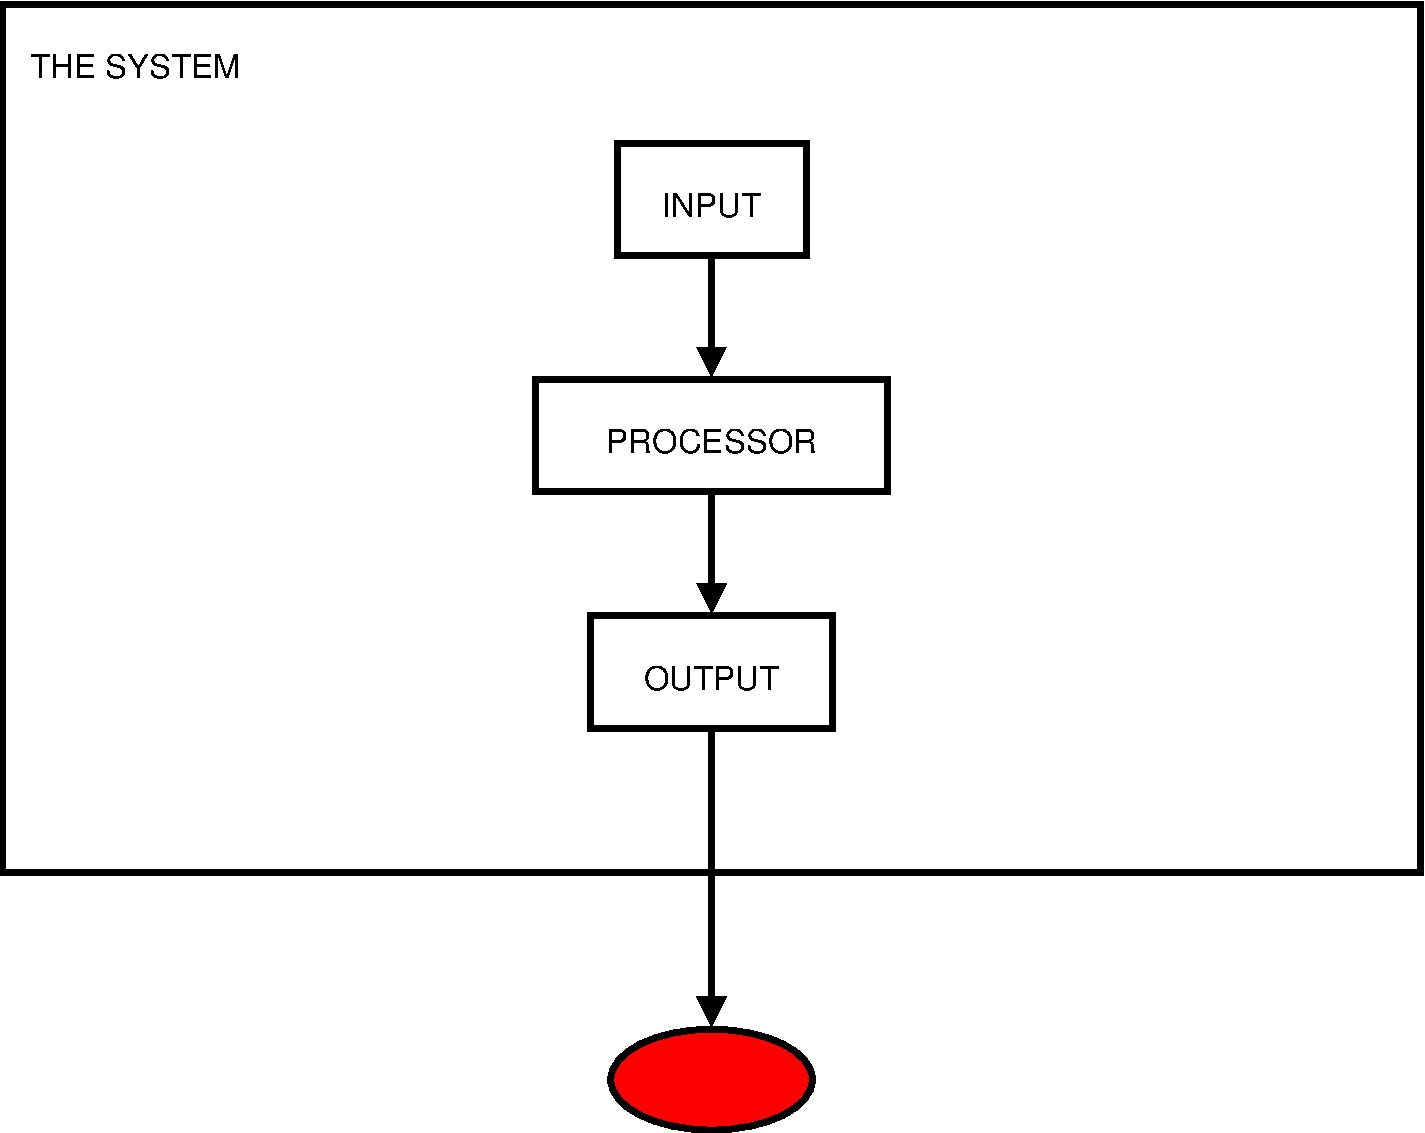
\includegraphics[width=.50\textwidth]{figures/example}
    \caption{An example image.}
    \label{fig:EXAMPLE1}
\end{figure}
\end{verbatim}

\noindent and

\begin{flushleft}
\small
\begin{verbatim}
\begin{table}[ht]
    \centering
    \caption{Table of values for $F(\chi)=\chi+4$.}
    \begin{tabular}[ht]{r|l}
        \hline
        $\chi$ & $F(\chi)=\chi+4$\\
        \hline
        $1$ & $5$\\
        $2$ & $6$\\
        $3$ & $7$\\
        $4$ & $8$\\
        \multicolumn{2}{l}{$\ldots$}\\
        \hline
    \end{tabular}
    \label{tab:EQUATION1_VALUES}.
\end{table}
\end{verbatim}
\end{flushleft}

\begin{figure}[ht]
    \centering
    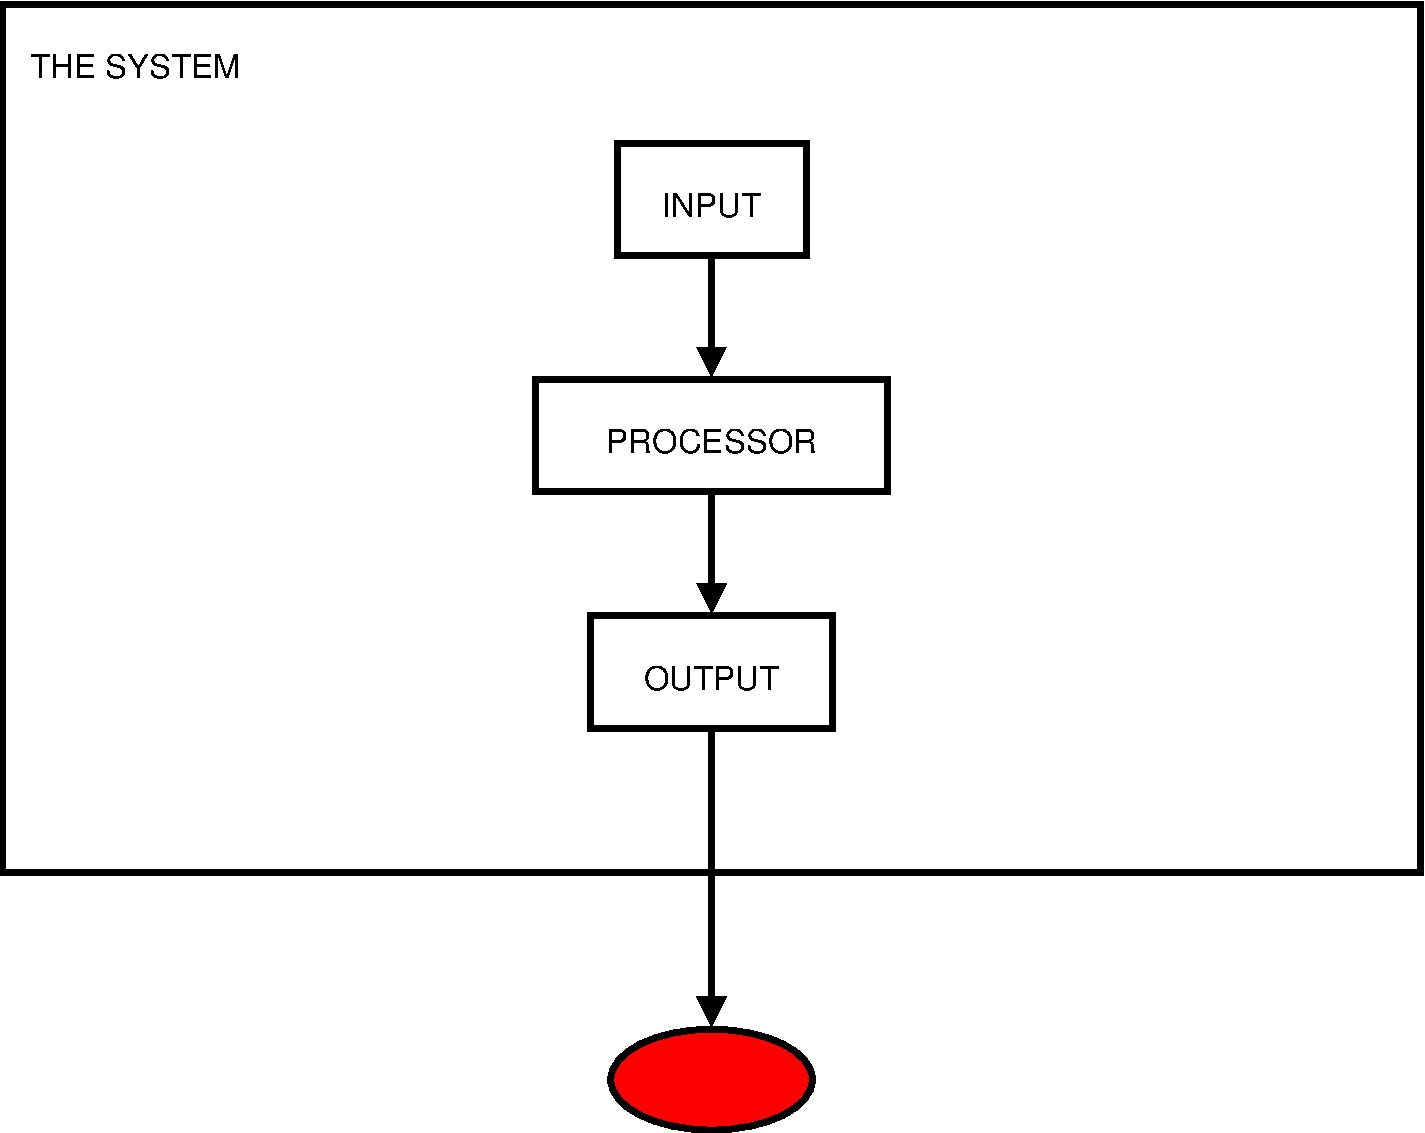
\includegraphics[width=.50\textwidth]{figures/example}
    \caption{An example image.}
    \label{fig:EXAMPLE1}
\end{figure}

\begin{table}[ht]
    \centering
    \caption{Table of values for $F(\chi)=\chi+4$.}
    \begin{tabular}[ht]{r|l}
	\hline
	$\chi$ & $F(\chi)=\chi+4$\\
	\hline
	$1$ & $5$\\
	$2$ & $6$\\
	$3$ & $7$\\
	$4$ & $8$\\
	\multicolumn{2}{l}{$\ldots$}\\
	\hline
    \end{tabular}
    \label{tab:EQUATION1_VALUES}.
\end{table}



We can also create \emph{sub}-figures (Figures~\ref{fig:MIX}
and~\ref{fig:BAKE}) and \emph{sub}-tables (Tables~\ref{tab:SUB1}
and~\ref{tab:SUB2}).  Look at the source for this chapter to see how
it was done, should you want to do it in your thesis.

\begin{figure}[!ht]
    \centering

    \subfloat[Make the Dough]{
    	\label{fig:MIX}
	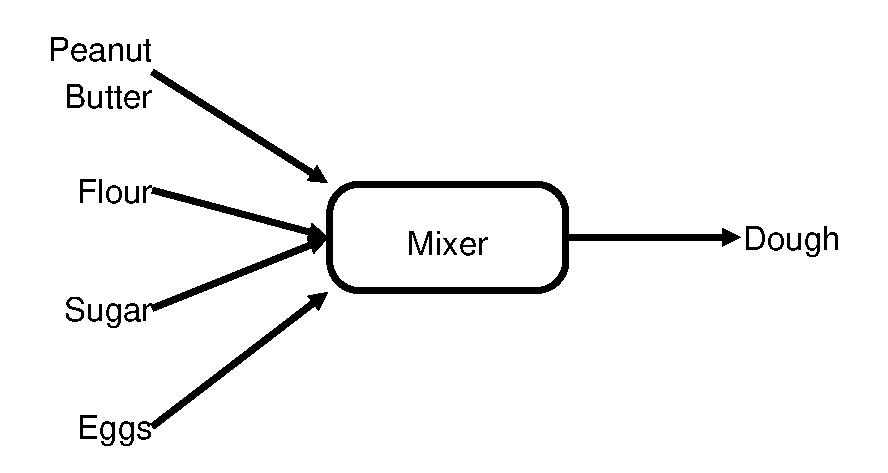
\includegraphics[width=0.45\textwidth]{figures/dough}
    }
     \subfloat[Bake the Cookies]{
    	\label{fig:BAKE}
	
\includegraphics[width=0.45\textwidth]{figures/oven}
    }
    \caption{Making Peanut Butter Cookies.}
    \label{fig:PEANUTBCOOKIES}
\end{figure}

\begin{table}[!ht]
    \centering
    \caption{Table of values for two other $F()$s.}
    \subfloat[$F(z)=x+y$]{
	\label{tab:SUB1}
	\begin{tabular}[ht]{lll}
    	    \hline
    	    $x$ & $y$&$F(z)=x+y$\\
	    \hline
	    $1$ & $2$ & $3$\\
	    $1$ & $3$ & $4$\\
	    $1$ & $4$ & $5$\\
	    $1$ & $5$ & $6$\\
	    $1$ & $6$ & $7$\\
	    \hline
    	\end{tabular}
    }
    \subfloat[$F(z)=x+2y$]{
	\label{tab:SUB2}
    	\begin{tabular}[ht]{lll}
    	    \hline
    	    $x$ & $y$&$F(z)=x+2y$\\
	    \hline
	    $1$ & $2$ & $5$\\
	    $1$ & $3$ & $7$\\
	    $1$ & $4$ & $9$\\
	    $1$ & $5$ & $11$\\
	    $1$ & $6$ & $13$\\
	    \hline
    	\end{tabular}
    }
    \label{tab:EQUATION2_VALUES}.
\end{table}


% This is an ugly way to get the tallstrut defn in the middle of the line.
% Speaking of things not being done the \LaTeX\ way...
% Maybe instead look at the last answer in
% http://tex.stackexchange.com/questions/24186/how-to-center-text-without-adding-space-and-not-altering-alignment-of-surroundin
You may have thought there wasn't enough space above and below the
line with $F(\chi)$ in Table~\ref{tab:EQUATION1_VALUES}.  JD certainly
doesn't think there is enough space there, and he feels that the fact
that \LaTeX's tabular environment doesn't automagically provide enough
space is a bit of a flaw.  JD uses plain \TeX\ rather than \LaTeX, and
thus doesn't know The One True \LaTeX\ Way to fix this, but he would
solve the problem by putting the definition

\begingroup
\leftskip=0cm plus 0.5fil
\rightskip=0cm plus -0.5fil
\parfillskip=0cm plus 1fil
\noindent
\verb|\def\tallstrut{\vrule width 0pt depth 5.5 pt height 12 pt}|
\par
\endgroup
\noindent
before the definition of the table and then changing
``\verb|$\chi$ & $F(\chi)=\chi+4$\\|'' in the table definition to read
``\verb|\tallstrut $\chi$ & $F(\chi)=\chi+4$\\|''.  This produces the
result shown in Table~\ref{tab:EQUATION1a_VALUES}.  The
\verb|depth 5.5pt| and \verb|height 12pt| tell \TeX\ to make sure
there is at least 5.5~pt.\ of space below the typesetting baseline and
12~pt.\ of space above the baseline.  If you decide to go to this
length to make your thesis look good (and why shouldn't you?\null),
keep in mind that you may wish to change these numbers, depending on
what characters are actually used on the line you are prettying up.

\def\tallstrut{\vrule width 0pt depth 5.5 pt height 12 pt}

\begin{table}[ht]
    \centering
    \caption{Table of values for $F(\chi)=\chi+4$.}
    \begin{tabular}[ht]{r|l}
	\hline
	\tallstrut $\chi$ & $F(\chi)=\chi+4$\\
	\hline
	$1$ & $5$\\
	$2$ & $6$\\
	$3$ & $7$\\
	$4$ & $8$\\
	\multicolumn{2}{l}{$\ldots$}\\
	\hline
    \end{tabular}
    \label{tab:EQUATION1a_VALUES}.
\end{table}

Finally, you should note that figures and tables should
\textbf{always} go \textbf{after} the first reference to them in the
text.  The ``\verb|[ht]|'' in the ``\verb|\begin{table}|'' line
indicates that you are happy with the figure going \verb|h|ere or at
the \verb|t|op of a following page.  (You can also use ``\verb|b|''
for the \verb|b|ottom of the page.)
Sometimes \LaTeX\ puts the float further away than necessary; if this
happens to you try changing ``\verb|[ht]|'' to  ``\verb|[!ht]|''. 
If you examine the source code for this chapter you will see this was
done in a couple of places.
